\newpage
\null

\begin{center}
    \Huge{\textbf{\underline{Chapter 2: Approached Resolution of}}} \\
    \vspace{0.25cm}
    \Huge{\textbf{\underline{Non-Linear Equation \( f(x) = 0 \)}}}
\end{center}

\setcounter{section}{0}

\vspace{0.35cm}
\section{\textbf{\protect\( \boldsymbol{f(x) = 0} \protect\)} Equation}

\begin{prettyBox}{\textbf{\protect\( \boldsymbol{f(x) = 0} \protect\)}}{mygreen}

Let \( \alpha \in \mathbb{R} \) such that \( f(\alpha) = 0 \).  

Graphically, \( f(x) = 0 \) means that the function \( f \) intersects the \( x \)-axis.  


In numerical methods, we approximate \( \alpha \) using a sequence \( (x_i) \) such that:  
\[
\alpha \approx x_i, \quad \text{for some } i
\]\end{prettyBox}


\vspace{0.35cm}


\begin{prettyBox}{Note}{red}
We use numerical methods only if the equation's degree is greater than \( 2 \)  
or if it is non-trivial, such as \( 3x - e^{-x} = 0 \).  
For linear or quadratic equations, exact methods are sufficient, and numerical methods are not needed.
\end{prettyBox}


\vspace{0.5cm}
\section{Sequence}
\begin{prettyBox}{Sequence}{mygreen}
Each numerical algorithm (method) has their specific sequence that must
convegre to the deseried solution
\end{prettyBox}

\vspace{0.5cm}
\section{Initial Steps Of Any Numerical Algorithm}

\begin{prettyBox}{Initial Steps}{mygreen}
Every numerical algorithm must first go through two crucial steps:  
\begin{enumerate}
    \item Determine the number of solutions.  
    \item Define the range of each solution within a closed, bounded, and continuous interval \([a, b]\).  
\end{enumerate}
\end{prettyBox}

\newpage

\begin{prettyBox}{Note}{red}
\begin{itemize}
    \item \textbf{Terminal Phase:} In numerical analysis, we aim for real
numerical values rather than exact expressions in fractional or functional form.  
    \item \textbf{Differences Between Algorithms:} The main difference between 
numerical algorithms lies in how they approximate and compute solution values
for each interval identified in the initial step.  
    \item \textbf{Exercises That Do Not Mention the Initial Steps:} Even if
an exercise does not explicitly state the need for the initial steps, we must
always perform them, as they are crucial regardless of the algorithm used.

\end{itemize}
\end{prettyBox}

\vspace{0.5cm}

\subsection{Finding the Number of Solutions}
\begin{prettyBox}{Number of Solutions}{mygreen}
To determine the number of solutions, we first analyze the \textbf{monotonicity} of the function and construct its \textbf{variation table}.  
Then, we apply the \textbf{Intermediate Value Theorem (IVT)} corollary to determine the number of roots: \\[0.15cm]

If \( f: I \to \mathbb{R} \) is \textbf{continuous} on the \textbf{closed and bounded interval} \([a, b]\) :
\begin{itemize}
    \item \( f(a) \cdot f(b) < 0 \) :
        \begin{itemize}
    \item \textbf{No monotonicity} → At least one root exists.
    \item \textbf{Strictly monotonic} → Exactly one root exists.
        \end{itemize}
    \item \( f(a) \cdot f(b) > 0 \) :
        \begin{itemize}
    \item 0 or even number of solution
        \end{itemize}
\end{itemize}
\end{prettyBox}

\vspace{0.5cm}


\subsection{Range for Each Solution}
\begin{prettyBox}{Range}{mygreen}
 Sometimes, key points can be found by differentiating.  
 If not, we can reduce the range by testing values,  
 ideally until the interval length reaches 1 for better performance.
\end{prettyBox}

\newpage

\textbf{\underline{Example :}}

\[f(x) = e^{-x} - \ln(x) = 0\]

\textbf{\underline{Finding Intervalle Of Definition}}
\begin{itemize}
    \item \(e^{-x}\)\hspace{0.2cm}is defined in \(\mathbb{R}\)
    \item \(ln(x)\)\hspace{0.2cm}is defined in \(]0,+\infty[\)
\end{itemize}

\[\boxed{D_{f} = \mathbb{R}\hspace{0.2cm}\cap\hspace{0.2cm}]0,+\infty[\hspace{0.2cm}=\hspace{0.2cm}]0,+\infty[}\]

\vspace{0.5cm}

\textbf{\underline{Differentiate}}\\[0.2cm]
Since \( f \) is the sum of two functions that are continuous and differentiable on \( D_f \) \(\Rightarrow\) \( f \) is also continious and differentiable on \( D_f \).


\[
f'(x) = -e^{-x} - \frac{1}{x} = -(e^{-x} + \frac{1}{x})
\]

\vspace{0.5cm}

Since \hspace{0.2cm}\( e^{-x} > 0 \) \hspace{0.2cm} and \hspace{0.2cm}\( \frac{1}{x} > 0 \) \hspace{0.2cm} \(\forall\) \hspace{0.2cm}\( x \in D_f\) = \(]0, +\infty[ \)\hspace{0.2cm} $\Rightarrow$  \hspace{0.2cm}\( e^{-x} + \frac{1}{x} > 0 \).  

\vspace{0.2cm}

Thus, \( f'(x) < 0 \) for all \( x \in D_f \), meaning \( f' \) is strictly negative and \( f \) is strictly decreasing on \( D_f \) (Montonic).

\vspace{1cm}

\textbf{\underline{Variation Table}}\\[0.25cm]

\begin{center}
 \begin{tikzpicture}
    \tkzTabInit{$x$/1, $f'(x)$/2 , $f(x)$/2}{$0$,$1$,$2$,$+\infty$}
    \tkzTabLine{,,,-,,}
    \tkzTabVar{+/$+\infty$ ,R/,R/, -/$-\infty$}
\end{tikzpicture}
\end{center}

\vspace{0.5cm}
\(f(1) \approx 0.36 > 0 \) , \(f(2) \approx -0.55 < 0\)

\vspace{1cm}
\textbf{\underline{IVT}}\\[0.25cm]
\(f\) is continuous and strictly montonic in \(I\) = \([1,2]\) , and \(f(1)\cdot f(2) < 0\) \(\Rightarrow\) Exactly one root

\newpage
\null

\section{Algorithm (Building The Sequence)}
\subsection{Dichotomy (Bisection)}
\begin{prettyBox}{Condition}{mygreen}
This method is based on the \textbf{Intermediate Value Theorem (IVT)} and therefore requires the function \( f \) to be continuous.  
Additionally, we need a closed and bounded interval \([a, b]\) that contains a \textbf{single} root \( \alpha \in [a, b] \).
\end{prettyBox}

\vspace{0.25cm}

\subsubsection{Order Of Convergence}
\begin{prettyBox}{Order}{mygreen}
The bisection method has a \textbf{linear order of convergence} : 1 , meaning the error decreases at a constant rate in each iteration.  
\end{prettyBox}

\vspace{0.25cm}
\subsubsection{Guaranteed Convergence}
\begin{prettyBox}{Guarantee}{mygreen}
Even though the bisection method is slow, it always guarantees to converge to the desired solution.
\end{prettyBox}

\vspace{0.25cm}
\subsubsection{Sequence}
\begin{prettyBox}{Sequence}{mygreen}
For each iteration, we divide the interval \([a_n,b_n]\) into two equal sub-intervals,
where \([a_0,b_0] = [a,b]\) and the midpoint is given by:
\[
    \boxed{x_n = \frac{a_n + b_n}{2} \hspace{0.2cm}, \hspace{0.2cm} \forall n \geq 0}
\]
For each iteration, we determine the correct sub-interval for the next step:
\begin{itemize}
    \item If \( f(a_n) \cdot f(x_n) < 0 \), then \( \alpha \in [a_n, x_n] \), so we set:
    \[
    [a_{n+1}, b_{n+1}] = [a_n, x_n]
    \]
    \item If \( f(b_n) \cdot f(x_n) < 0 \), then \( \alpha \in [x_n, b_n] \), so we set:
    \[
    [a_{n+1}, b_{n+1}] = [x_n, b_n]
    \]
\end{itemize}
\end{prettyBox}

\vspace{0.25cm}
\subsubsection{Error Estimation}
\begin{prettyBox}{Error Estimation}{mygreen}
\begin{center}
    \boxed{E_n = |\alpha - x_n| \leq \frac{b-a}{2^{n+1}} \hspace{0.2cm}, \hspace{0.2cm} \forall n \geq 0}
\end{center}
\end{prettyBox}

\vspace{0.15cm}

\subsubsection{Tolerance}
\begin{prettyBox}{Tolerance}{mygreen}
Tolerance is a fixed value set by the user to ensure that the error does not exceed a predefined bound, denoted by \(\epsilon\).
\begin{center}
\boxed{E_n = |\alpha - x_n| \leq \frac{b-a}{2^{n+1}} \leq \epsilon \hspace{0.2cm}, \hspace{0.2cm} \forall n \geq 0}
\end{center}
\end{prettyBox}

\vspace{0.15cm}


\subsubsection{Number Of Iterations}
\begin{prettyBox}{Number Of Iterations}{mygreen}
    
    \begin{center}
    \[
    \begin{gathered}
        \epsilon \geq \dfrac{b-a}{2^{n+1}} \\[0.3cm]
        \dfrac{2^{n+1}}{b-a} \geq \dfrac{1}{\epsilon} \\[0.3cm]
        2^{n+1} \geq \dfrac{b-a}{\epsilon} \\[0.3cm]
        \ln(2^{n+1}) \geq \ln\left(\dfrac{b-a}{\epsilon}\right) \\[0.3cm]
        (n+1) \ln(2) \geq \ln\left(\dfrac{b-a}{\epsilon}\right) \\[0.3cm]
        n \geq \dfrac{\ln\left(\dfrac{b-a}{\epsilon}\right)}{\ln(2)} - 1 \\[0.3cm]
        \boxed{n = \left\lceil \dfrac{\ln\left(\dfrac{b-a}{\epsilon}\right)}{\ln(2)} - 1 \right\rceil}
    \end{gathered}
    \]
    \end{center}
\end{prettyBox}
\vspace{0.25cm}

\subsubsection{Solution Intervalle}
\begin{prettyBox}{Solution Intervalle}{mygreen}
    \begin{center}
    \[
    \begin{gathered}
        |\alpha - x_n| \leq \epsilon \\[0.3cm]
        -\epsilon \leq \alpha - x_n \leq \epsilon \\[0.3cm]
        \boxed{x_n - \epsilon \leq \alpha \leq \epsilon + x_n}\\[0.3cm]
    \end{gathered}
    \]
    \end{center}
\end{prettyBox}


\vspace{0.5cm}

\begin{prettyBox}{Note}{red}
\begin{itemize}
    \item The number of iterations is affected by the length of the interval \([a, b]\).  
          By convention, it is better to choose an interval of length 1 for better performance.
    \item Length of an interval \([a, b]\): \(b - a\).
    \item Midpoint (bisection) of an interval \([a, b]\): \(\dfrac{a + b}{2}\).
\item Some exercises may not provide the problem directly, requiring us to model it.
\end{itemize}
\end{prettyBox}

\vspace{1cm}

\textbf{\underline{Example}}\\[0.2cm]
approximate the value of \(\sqrt[3]{80}\) with the tolerance \(\epsilon = 10^{-1}\)

\vspace{1cm}

\textbf{\underline{Modelisation Of The Problem}}\\[0.2cm]
\[x = \sqrt[3]{80} \Rightarrow x^3 = 80 \Rightarrow \boxed{f(x) = x^3 - 80}\]

\vspace{1cm}
\textbf{\underline{Finding Intervalle Of Definition}}\\[0.2cm]
\begin{center}
Since \(f\) is a polynomial function \(\Rightarrow \boxed{D_f = \mathbb{R}}\)
\end{center}

\newpage
\textbf{\underline{Differentiate}}\\[0.2cm]
Since \(f\) is a polynomial function, it's continuous and differentiable on \(D_f\).

\vspace{0.35cm}
\begin{center}
\(f'(x) = 3x^2\)\\[0.3cm]
\(f'(0) = 0\)
\end{center}

\vspace{0.35cm}
Since \(f'(x) \geq 0\) on \(D_f \Rightarrow f\) is increasing on \(D_f\) (monotonic)

\vspace{1cm}

\textbf{\underline{Variation Table}}\\[0.25cm]

\begin{center}
 \begin{tikzpicture}
    \tkzTabInit{$x$/1, $f'(x)$/2 , $f(x)$/2}{$-\infty$,$0$,$4$,$5$,$+\infty$}
    \tkzTabLine{,+,z,,,+,}
    \tkzTabVar{-/$-\infty$ ,R/,R/,R/, +/$+\infty$}
\end{tikzpicture}
\end{center}

\vspace{0.5cm}

\(f(0) = -80\), which means that \(\alpha \in [0,+\infty[\).  
We are going to shorten the interval by testing the points \(4\) and \(5\):  
\(f(4) = -16\) and \(f(5) = 45\).

\vspace{1cm}
\textbf{\underline{Intermediate Value Theorem (IVT)}}\\[0.25cm]
Since \(f\) is continuous and strictly monotonic in \(I = [4,5]\), and \(f(4) \cdot f(5) < 0\),  
\(\Rightarrow\) There exists exactly one root in the interval \([4,5]\).

\vspace{0.35cm}

\textbf{\underline{Number Of Iteration}}\\[0.25cm]

\begin{center}
\(n = \left\lceil \dfrac{\ln\left(\dfrac{b-a}{\epsilon}\right)}{\ln(2)} - 1 \right\rceil = \left\lceil \dfrac{\ln\left(\dfrac{5-4}{10^{-1}}\right)}{\ln(2)} - 1 \right\rceil = \boxed{\left\lceil 2.3 \right\rceil = 3}\)
\end{center}

\newpage
\textbf{\underline{Bisection}}\\[0.15cm]
\textbf{\underline{Iterration 1}}
\begin{center}
    \(x_0 = \dfrac{a_0+b_0}{2} = \dfrac{4+5}{2} = \dfrac{9}{2} = 4.5\)\\[0.4cm]
    \(f(x_0) = f(4.5) = 11.125\)\\[0.4cm]
    \(f(x_0) . f(a_0) < 0 \Rightarrow [a_1,b_1] = [a_0,x_0] =[4,4.5] \)
\end{center}

\vspace{0.8cm}

\textbf{\underline{Iterration 2}}
\begin{center}
    \(x_1 = \dfrac{a_1+b_1}{2} = \dfrac{4+4.5}{2}= \dfrac{17}{4} = 4.25\)\\[0.4cm]
    \(f(x_1) = f(4.25)  \approx -3.2\)\\[0.4cm]
    \(f(x_1) . f(b_1) < 0 \Rightarrow [a_2,b_2] = [x_1,b_1] = [4.25,4.5]\)
\end{center}

\vspace{0.8cm}

\textbf{\underline{Iterration 3}}
\begin{center}
    \(x_2 = \dfrac{a_2+b_2}{2} = \dfrac{4.5+4.25}{2} =\dfrac{35}{8} = 4.375\)\\[0.4cm]
    \(f(x_2) = f(4.375)  \approx 3.74\)\\[0.4cm]
    \(f(x_2) . f(a_2) < 0 \Rightarrow [a_3,b_3] = [a_2,x_2] = [4.25,4.375]\)
\end{center}

\vspace{0.8cm}

\textbf{\underline{Iterration 4}}
\begin{center}
    \(x_3 = \dfrac{a_3+b_3}{2} = \dfrac{4.25+4.375}{2} =\dfrac{69}{16} = 4.3125\)\\[0.4cm]
\end{center}

\vspace{1cm}


\textbf{\underline{Error Estimation}}
\begin{center}
    \(E_3 = \dfrac{b-a}{2^{3+1}} = \dfrac{5-1}{2^4} = \dfrac{1}{16} = \boxed{0.0625 < \epsilon = 10^{-1}}\) 
\end{center}

\vspace{0.3cm}
\textbf{\underline{Solution Interval}}
\begin{center}
   \(x_3 - \epsilon \leq \alpha \leq x_3 + \epsilon\)\\[0.1cm]
   \(\boxed{4.3125 - 10^{-1} \leq \alpha \leq 4.3125 + 10^{-1}}\)\\[0.1cm]
\end{center}

\vspace{0.2cm}
\textbf{\underline{Conclusion}}
\begin{center}
    \(\boxed{\alpha = \sqrt[3]{80} \approx x_3 = 4.3125}\)
\end{center}

\subsection{Fixed Point \(\varphi\)}
\begin{prettyBox}{Fixed Point}{mygreen}
Let \( f \) be a continuous function on \([a, b]\) and \(\exists!\alpha \in [a, b]\) such that:
\[
f(\alpha) = 0 \iff \varphi(\alpha) = \alpha.
\]

\vspace{0.15cm}

This method consists of transforming the equation \( f(x) = 0 \) into:

\begin{center}
    \(\boxed{\varphi(x) = x}\)
\end{center}

\vspace{0.15cm}
Our goal is to find a suitable function \(\varphi\) related to \( f \) , we will
learn about the conditions on \(\varphi\) in the next section.\\[0.1cm]
Graphically, this corresponds to the intersection of \(\varphi\) with the first bisector \( y = x \).
\end{prettyBox}

\vspace{0.5cm}
\begin{prettyBox}{Note}{red}
\begin{itemize}
    \item A function \( f \) may have more than one possible choice for 
\(\varphi\).
    \item Each root of \( f \) corresponds to a different function \(\varphi\).
\end{itemize}
\end{prettyBox}

\vspace{1cm}
\textbf{\underline{Example}}
\begin{center}
\(f(x) = e^{x} - 2x - 1 = 0\)
\end{center}

\vspace{0.25cm}

\begin{center}
    \(e^{x} - 1 = 2x\)\\[0.1cm]
    \(e^{x} = 2x + 1\)\\[0.1cm]
    \(\boxed{x = \ln(2x+1) = \varphi_{1}}\)
\end{center}

\vspace{0.25cm}

\begin{center}
    \(-2x - 1 = -e^{x}\)\\[0.1cm]
    \(-2x = -e^{x} + 1\)\\[0.1cm]
    \(\boxed{x = \dfrac{e^{x} - 1}{2} = \varphi_{2}}\)
\end{center}

\vspace{0.75cm}
\subsection{Conditions for Choosing the Right \(\varphi\)}
\begin{prettyBox}{Conditions}{mygreen}
As seen in the previous example, a function \( f \) can have more than one
possible \(\varphi\). The necessary conditions for choosing a suitable 
\(\varphi\) are:  
\begin{itemize}
    \item \textbf{Stability}
    \item \textbf{Contraction}
\end{itemize}
\end{prettyBox}

\vspace{0.6cm}
\subsubsection{Stability}
\begin{prettyBox}{Stability}{mygreen}
Let \(\varphi\) be defined on \([a, b]\) , \(\varphi\) is stable if and only if :
\begin{center}
    \(\varphi([a, b]) \subseteq [a, b]\)
\end{center}

\vspace{0.1cm}
To check whether this is true, we need the table of variations of \(\varphi\). 
By differentiating it (\(\varphi'\)), we can determine the critical points and
analyze the behavior of \(\varphi\). 
Then, we need to verify if the maximum and minimum values of \(\varphi\) on 
\([a, b]\) lie within \([a, b]\).
\end{prettyBox}

\vspace{0.5cm}
\subsubsection{Contraction}
\begin{prettyBox}{Contraction}{mygreen}
Let \(\varphi\) be defined on \([a, b]\) , \(\varphi\) is contracted if 
\(\exists k \in ]0,1[\) such that

\begin{center}
 \(|\varphi(x) - \varphi(y)| \leq k\cdot|x-y| \hspace{0.2cm} \forall x,y 
\in[a,b]\)
\end{center}

\vspace{0.1cm}
To check constraction of \(\varphi\) we use the following result :\\[0.1cm]
If \(\varphi\) is defined in \([a,b]\) and \(\varphi \in C^{1} \) :
\begin{align*}
    \sup_{x \in [a, b]} |\varphi'(x)| < 1 &\Longrightarrow \text{Contractive}\\[0.1cm]
    \sup_{x \in [a, b]} |\varphi'(x)| \geq 1 &\Longrightarrow \text{Not Contractive}
\end{align*}
\vspace{0.1cm}

We need to study variation of \(\varphi'\) to retrieve
the min and max in \([a,b]\) to get the sup value.
\end{prettyBox}

\vspace{0.5cm}


\subsection{Sequence}
\begin{prettyBox}{Sequence}{mygreen}
    Let \(\varphi\) be continuous, stable, and contractive on \([a,b]\), we have:\\[0.15cm]
    \(\exists! \alpha \in [a,b]\) solution of \(\varphi(x) = x\).\\[0.1cm]
\(\forall x_0 \in [a,b]\), the sequence \(x_n\) is defined \(\forall n \geq 0\) by:

\begin{center}
  \(x_{n+1} = \varphi(x_n)\), which converges to \(\alpha\).
\end{center}
\end{prettyBox}

\subsection{Error Estimation}
\begin{prettyBox}{Error Estimation}{mygreen}
\begin{center}
    \(\boxed{|x_n - \alpha| \leq \dfrac{k^{n}}{1-k} \cdot |x_1-x_0| \hspace{0.2cm} \forall n\geq 0}\)
\end{center}
\end{prettyBox}

\vspace{0.5cm}

\subsection{Tolerance}
\begin{prettyBox}{Tolerance}{mygreen}
\begin{center}
    \(\boxed{|x_n - \alpha| \leq \dfrac{k^{n}}{1-k} \cdot |x_1-x_0| \leq \epsilon \hspace{0.2cm} \forall n\geq 0}\)
\end{center}
\end{prettyBox}



\vspace{0.5cm}

\subsubsection{Number Of Iterations}
\begin{prettyBox}{Number Of Iterations}{mygreen}
    
    \begin{center}
    \[
    \begin{gathered}
        \epsilon \geq \dfrac{k^{n}}{1-k} \cdot |x_1-x_0| \\[0.3cm]
         k^{n} \cdot |x_1 - x_0| \leq \epsilon \cdot (1-k)   \\[0.3cm]
         k^{n}  \leq \dfrac{\epsilon \cdot (1-k)}{|x_1 - x_0|}   \\[0.3cm]
         \ln(k^{n}) \leq \ln\left(\dfrac{\epsilon \cdot (1-k)}{|x_1 - x_0|}\right)   \\[0.3cm]
         n\cdot\ln(k) \leq \ln\left(\dfrac{\epsilon \cdot (1-k)}{|x_1 - x_0|}\right)   \\[0.3cm]
         n \geq \dfrac{\ln\left(\dfrac{\epsilon \cdot (1-k)}{|x_1 - x_0|}\right)}{\ln(k)}   \\[0.3cm]
         \boxed{n =  \left\lceil \dfrac{\ln\left(\dfrac{\epsilon \cdot (1-k)}{|x_1 - x_0|}\right)}{\ln(k)}\right\rceil}   \\[0.3cm]
    \end{gathered}
    \]
    \end{center}
\end{prettyBox}
\vspace{0.25cm}



\vspace{0.5cm}
\subsection{Proof}
\subsubsection{Existence \& Uniqueness Of Solution \(\alpha\)}
\begin{prettyBox}{Existence \& Uniqueness}{mygreen}
\textbf{\underline{Existence:}}\\[0.2cm]
Let the function \(h\) be continuous on \([a,b]\) : \(h(x) = \varphi(x) - x\).
We have:

\vspace{-0.6cm}
\begin{center}
\[
\left\{
\begin{array}{ll}
   h(a) = \varphi(a) - a \geq 0 \\[0.1cm]
   h(b) = \varphi(b) - b \leq 0
\end{array}
\right.
\]
\end{center}

From the Intermediate Value Theorem (IVT), \(h\) has at least one root \(\alpha \in [a,b]\) such that  
\(h(\alpha) = 0 \Longrightarrow \varphi(\alpha) = \alpha\).

\vspace{0.4cm}

\textbf{\underline{Uniqueness:}}\\[0.2cm]
Suppose there exists another root \(\beta \in [a,b]\). Using the contraction property for
\(\alpha\) and \(\beta\), we get:
\vspace{0.1cm}
\begin{center}
    \(|\varphi(\beta) - \varphi(\alpha)| \leq k\cdot|\beta-\alpha|\)\\[0.2cm]
    \(|\beta - \alpha| \leq k\cdot|\beta-\alpha|\)
\end{center}
Contradiction, since \(k \in ]0,1[\), then:
\begin{center}
      \(|\beta - \alpha| > k\cdot|\beta-\alpha|\)\\[0.1cm]
\end{center}
Therefore, the solution is unique.
\end{prettyBox}

\vspace{0.5cm}


\subsubsection{Convergence to \(\alpha\)}
\begin{prettyBox}{Convergence}{mygreen}
Since \(\varphi\) is stable and continuous on \([a,b]\), we have:
\[
\forall n \geq 0, \quad x_n \in [a,b]
\]
Assume that \(x_n\) converges to some limit \( l \in [a,b] \).

\begin{center}
    \(\lim\limits_{n \to \infty} x_{n+1} = \lim\limits_{n \to \infty} \varphi(x_n)\)\\[0.15cm]
    \(l = \varphi(\lim\limits_{n \to \infty} x_n)\)\\[0.15cm]
    \(\boxed{l = \varphi(l)}\) 
\end{center}

Thus, \( l = \alpha \).\\[0.15cm]
Now, we will prove that \(x_n\) indeed converges to the fixed point \(\alpha\).  
Since \(\varphi\) is contractive, we obtain:

\begin{center}
    \(|x_n - \alpha| = |\varphi(x_{n-1}) - \varphi(\alpha)| \leq k\cdot|x_{n-1}-\alpha|\)\\[0.15cm] 
    \(|x_{n-1} - \alpha| = |\varphi(x_{n-2}) - \varphi(\alpha)| \leq k\cdot|x_{n-2}-\alpha|\)\\[0.15cm]
    \(k\cdot|x_{n-1} - \alpha|  \leq k\cdot k\cdot|x_{n-2}-\alpha|\)\\[0.15cm]
    \(k\cdot|x_{n-1} - \alpha|  \leq k^2\cdot|x_{n-2}-\alpha|\)\\[0.15cm]
    \(|x_n - \alpha| \leq k\cdot|x_{n-1} - \alpha|  \leq k^2\cdot|x_{n-2}-\alpha| \leq \dots \leq k^n \cdot |x_0 - \alpha|\)\\[0.15cm]
    \(\boxed{0 \leq |x_n - \alpha| \leq k^n \cdot |x_0 - \alpha|}\)
\end{center}
\vspace{0.15cm}
Taking the limit as \( n \to \infty \), we note that \( k^n \to 0 \) since \( k < 1 \), therefore:

\begin{center}
    \(\lim\limits_{n \to \infty} |x_n - \alpha| = 0\)\\[0.1cm]
    \(\boxed{\lim\limits_{n \to \infty} x_n = \alpha}\)
\end{center}

Thus, \( x_n \) converges to \( \alpha \).
\end{prettyBox}

\vspace{0.45cm}
\subsubsection{Error}
\begin{prettyBox}{Error}{mygreen}
Since \(\varphi\) is contractive, we obtain:

\begin{center}
    \(|x_{n+1} - x_n| = |\varphi(x_n) - \varphi(x_{n-1})| \leq k\cdot|x_{n}- x_{n-1}|\)\\[0.15cm] 
    \(|x_{n+1} - x_n| \leq k\cdot|x_{n} - x_{n-1}|  \leq k^2\cdot|x_{n-1}- x_{n-2}| \leq \dots \leq k^n \cdot |x_1 - x_0|\)\\[0.15cm]
    \(\boxed{|x_{n+1} - x_{n}| \leq k^n \cdot |x_1 - x_0|} \hspace{1cm} \text{(1)}\)
\end{center}

Let \(m \gg n\):
\begin{center}
    \(|x_{m} - x_{n}| =  |x_m - x_{m-1} + x_{m-1} - \dots - x_{n+1} + x_{n+1} - x_n|\)
\end{center}

Using the triangle inequality \(|a+b| \leq |a| + |b|\), we get:

\begin{center}
    \(\boxed{|x_{m} - x_{n}| \leq  |x_m - x_{m-1}| + |x_{m-1} - x_{m-2}| + \dots + |x_{n+1} - x_n|} \hspace{1cm} \text{(2)}\)
\end{center}

Replacing (1) in (2):

\begin{center}
    \(|x_{m} - x_{n}| \leq k^{m-1} \cdot|x_1 - x_0| + k^{m-2}\cdot |x_{1} - x_{0}| + \dots + k^{n}\cdot| x_{1} - x_0|\)\\[0.15cm]
    \hspace{-1.5cm} \(\leq [k^{m-1} + k^{m-2} + \dots + k^{n}] \cdot| x_{1} - x_0|\)\\[0.15cm]
    \hspace{-2.9cm}\(\leq k^{n} \cdot \left[\sum\limits_{j=0}^{m-n-1} k^j \right] \cdot| x_{1} - x_0|\)
\end{center}

Using the geometric series formula for \(N\) terms with \(r \neq 1\):
\begin{center}
    \(S = a + a\cdot r + a\cdot r^2 + \dots + a\cdot r^{N-1}\)\\[0.2cm]
    \(S = a\cdot \dfrac{1-r^{N}}{1-r}\)
\end{center}

Setting \(N = m-n\):

\begin{center}
    \(|x_m - x_n| \leq k^{n} \cdot \dfrac{1-k^{m-n}}{1-k} \cdot| x_{1} - x_0|\)
\end{center}

As \(m \to \infty\), \(x_m\) converges to \(\alpha\) and \(k^{m-n}\) converges to 0:

\begin{center}
    \(\boxed{|x_n - \alpha| \leq \dfrac{k^n}{1-k} \cdot| x_{1} - x_0|}\)
\end{center}
\end{prettyBox}

\newpage

\begin{prettyBox}{Note}{red}
When a function \(\varphi\) does not satisfy the required conditions, there are two possible cases:  
\begin{itemize}
    \item \textbf{Incorrect interval \([a, b]\):} The function \(\varphi\) may have issues at one or both endpoints. In such cases, choosing a slightly smaller interval \([a', b']\) can resolve the problem.  
    \item \textbf{Incorrect function \(\varphi\):} The issue may lie not in the interval but in the function itself when \(\displaystyle\inf_{x \in [a, b]} |\varphi'(x)| \geq 1\).  
\end{itemize}


Sometimes, there may be multiple functions \(\varphi\) that satisfy all the conditions on \([a, b]\). In such cases, we choose the one with the smallest contraction factor, as it ensures faster convergence:  

\[
\min \left( \sup_{x \in [a, b]} |\varphi_n'(x)| \right)
\]
\end{prettyBox}

\vspace{0.75cm}

\textbf{\underline{Example:}}
\[
f(x) = x + 1 - \frac{x\cdot e^{x}}{3} \hspace{0.4cm}, \quad D_f = \mathbb{R} \hspace{0.4cm}, \quad \epsilon = 10^{-4}\]

\vspace{0.5cm}
\textbf{\underline{Differentiation}}\\[0.2cm]
\( f \) is continuous and differentiable on \( D_f \).

\begin{center}
    \begin{align*}
        &f'(x) = 1 - \dfrac{1}{3}(e^{x}+x\cdot e^{x})\\[0.1cm] 
        &\boxed{f'(x) = 1 - \dfrac{e^{x}}{3}(1+x)}
    \end{align*}
\end{center}

\vspace{1cm}

Since \( f' \) is ambiguous, we can't study its sign; therefore, we need to analyze \( f'' \).  
\( f' \) is continuous and differentiable on \( D_f \).

\begin{center}
    \begin{align*}
        &f''(x) =  - \dfrac{1}{3}(e^{x}+e^{x}+x\cdot e^{x})\\[0.1cm] 
        &\boxed{f''(x) =  \dfrac{-e^{x}}{3}(2+x)}\\[0.1cm]
        &\boxed{f''(-2) = 0}
    \end{align*}
\end{center}

\newpage
\textbf{\underline{Variation Table}}

\begin{center}
 \begin{tikzpicture}
     \tkzTabInit{$x$/1, $f''(x)$/1 , $f'(x)$/2, $f'(x)$/1, $f(x)$/2}
     {$-\infty$, $-2$, $\beta$, $+\infty$}
    \tkzTabLine{,+,z,,-,}
    \tkzTabVar{-/$1$ ,+/1.045, R/, -/$-\infty$}
    \tkzTabLine{,,+,,z,-}
    \tkzTabVar{-/$-\infty$, R/, +/$f(\beta)$, -/$-\infty$}
\end{tikzpicture}
\end{center}

\vspace{0.5cm}

We evaluate \( f(x) \) at specific points starting from -2:

\vspace{0.25cm}
\begin{center}
 \( f(-2) = -0.90 < 0, \quad f(-1) = 0.1226 > 0, \quad f(1) = 1.09 > 0, \quad f(2) = -1.92 < 0\)
\end{center}

\vspace{0.35cm}

By the \textbf{Intermediate Value Theorem (IVT)}, since \( f(x) \) is monotonic continious and changes sign in the intervals \( [-2, -1] \) and \( [1,2] \), there exist two real roots:

\begin{center}
    \(\boxed{\alpha_1 \in [-2, -1], \quad \alpha_2 \in [1, 2]}\)
\end{center}

\vspace{1cm}
\textbf{\underline{Finding \(\varphi\) Functions}}

\begin{center}
    \(x+1 - \dfrac{x\cdot e^{x}}{3} = 0\)\\[0.15cm]
    \(\boxed{x =  \dfrac{x\cdot e^{x}}{3} -1  = \varphi_1}\)\\[0.75cm]
    \(x (1 - \dfrac{e^{x}}{3}) + 1 = 0\)\\[0.2cm]
    \(x (1 - \dfrac{e^{x}}{3})  = - 1\)\\[0.2cm]
    \(\boxed{x = \dfrac{1}{\frac{e^{x}}{3}-1} = \dfrac{1}{\frac{e^{x} - 3}{3}} = \dfrac{3}{e^{x}-3} = \varphi_2}\)\\[0.15cm]
\end{center}

\newpage
\begin{center}
\(\dfrac{x\cdot e^{x}}{3} = x+1\)\\[0.2cm]
\(\boxed{x = \dfrac{3(x+1)}{e^{x}} = \varphi_3}\)\\[0.5cm]
\(e^{x} = \dfrac{3(x+1)}{x}\)\\[0.2cm]
\(\boxed{x = \ln{\left(\dfrac{3(x+1)}{x}\right)} = \varphi_4}\)\\[0.2cm]
\end{center}

\vspace{1cm}
\textbf{\underline{Checking \(\varphi_1\)}}\\[0.15cm]
\textbf{\underline{\(D_{\varphi_1}\)}}
\begin{center}
    \( \boxed{D_{\varphi_1} = \mathbb{R}}\)
\end{center}
\textbf{\underline{\(\varphi_1'\)}}
\begin{center}
    \begin{align*}
        &\varphi_1'(x) = \dfrac{1}{3} (x\cdot e^{x} + e^{x})\\[0.15cm]
        &\boxed{\varphi_1'(x) = \dfrac{e^{x}}{3} (x + 1)}\\[0.15cm]
        &\boxed{\varphi_1'(-1) = 0}
    \end{align*}
\end{center}

\vspace{0.5cm}
\textbf{\underline{\(\varphi_1''\)}}
\begin{center}
    \begin{align*}
        &\varphi_1''(x) = \dfrac{1}{3} (e^{x}+e^{x}+x\cdot e^{x})\\[0.15cm]
        &\boxed{\varphi_1''(x) = \dfrac{e^{x}}{3} (x + 2)}\\[0.15cm]
        &\boxed{\varphi_1''(-2) = 0}
    \end{align*}
\end{center}

\newpage
\textbf{\underline{Variation Table}}

\begin{center}
 \begin{tikzpicture}
     \tkzTabInit {$x$/1, $\varphi_1''(x)$/1 , $\varphi_1'(x)$/2, $\varphi_1'(x)$/1, $\varphi_1(x)$/2}
     {$-2$, $-1$, $1$,$2$}
    \tkzTabLine{z,,,+,,}
    \tkzTabVar{-/$-0.045$ ,+/$0$, +/$1.81$, +/$7.98$}
    \tkzTabLine{,-,z,,+,}
    \tkzTabVar{+/$-1.09$, -/$-1.12$,+/-0.09, +/$5.9$}
\end{tikzpicture}
\end{center}
\vspace{0.25cm}

\(\displaystyle\inf_{x \in [1, 2]} |\varphi_1'(x)| = 1.81 > 1 \Longrightarrow \varphi_1\) is disqualified 
for the intervalle [1,2]

\vspace{0.5cm}
\(\varphi_1([-2,-1]) \subseteq [-2,-1] \Longrightarrow \varphi_1\) is stable on \([-2,-1]\)\\[0.1cm]
\( \varphi_1 \in C^{1} \text{ and } \displaystyle\sup_{x \in [-2, -1]} |\varphi_1'(x)| = 0.045 < 1 \Longrightarrow \varphi_1\) is contractive on \([-2,-1]\)

\begin{center}
    \(\boxed{\varphi_1 \text{ Corresponds to the root } \alpha_1 \in [-2,-1]}\)
\end{center}

\vspace{1cm}
\textbf{\underline{Checking \(\varphi_2\)}}\\[0.15cm]
\textbf{\underline{\(D_{\varphi_2}\)}}
\begin{center}
    \( \boxed{D_{\varphi_2} = \mathbb{R} - \{\ln{(3)}\}}\)
\end{center}

\textbf{\underline{\(\varphi_2'\)}}
\begin{center}
    \(\boxed{\varphi_2'(x) = \dfrac{-3e^{x}}{(e^{x}-3)^{2}}}\)\\[0.45cm]
    \(\boxed{\forall x \in D_{\varphi_2} \hspace{0.4cm} \varphi_2' < 0}\)
    \end{center}

\newpage
\textbf{\underline{\(\varphi_2''\)}}
\begin{center}
    \begin{align*}
        &\varphi_2''(x) = -3 \cdot \dfrac{e^{x}(e^x - 3)^2 - e^{x}(2e^x(e^x-3)^{2-1})}{(e^{x}-3)^4}\\[0.15cm]
        &\varphi_2''(x) = -3 \cdot \dfrac{e^{x}(e^x - 3) ((e^x - 3) - 2e^{x})}{(e^{x}-3)^4}\\[0.15cm]
        &\varphi_2''(x) = -3 \cdot \dfrac{e^{x} (- 3 -e^{x})}{(e^{x}-3)^3}\\[0.15cm]
        &\boxed{\varphi_2''(x) = 3 \cdot \dfrac{e^{x} (3 + e^{x})}{(e^{x}-3)^3}}\\[0.15cm]
    \end{align*}
\end{center}

\begin{center}
    \(\boxed{\forall x > \ln(3) \hspace{0.3cm} \varphi_2'' > 0}\)\\[0.15cm]
    \(\boxed{\forall x < \ln(3) \hspace{0.3cm} \varphi_2'' < 0}\)
\end{center}

\vspace{1cm}
\textbf{\underline{Variation Table}}

\begin{center}
 \begin{tikzpicture}
     \tkzTabInit {$x$/1, $\varphi_2''(x)$/1 , $\varphi_2'(x)$/2, $\varphi_2'(x)$/1, $\varphi_2(x)$/2}
     {$-2$, $-1$, $1$,$\ln(3)$,$2$}
    \tkzTabLine{,,-,,,,d,+,}
    \tkzTabVar{+/$-0.04$ ,-/$-0.15$,-/$-102.75$, -D-/ $-\infty$ / $-\infty$ , +/$-1.15$ }
    \tkzTabLine{,,-,,,,d,-,}
    \tkzTabVar{+/$-1.04$ ,-/$-1.35$,-/$-10.6$, -D+/ $-\infty$ / $+\infty$ , -/$0.68$ }
\end{tikzpicture}
\end{center}
\vspace{0.25cm}

\vspace{0.25cm}

\(\displaystyle\inf_{x \in [1,\ln{(3)}[} |\varphi_2'(x)| = 102.75 > 1 \Longrightarrow \varphi_2\) is disqualified 
for the intervalle \([1,\ln{(3)}[\)\\[0.15cm]
\(\displaystyle\inf_{x \in ]\ln{(3)},2]} |\varphi_2'(x)| = 1.15 > 1 \Longrightarrow \varphi_2\) is disqualified 
for the intervalle \(]\ln{(3)},2]\)

\vspace{0.5cm}
\(\varphi_2([-2,-1]) \subseteq [-2,-1] \Longrightarrow \varphi_2\) is stable on \([-2,-1]\)\\[0.1cm]
\( \varphi_2 \in C^{1} \text{ and } \displaystyle\sup_{x \in [-2, -1]} |\varphi_2'(x)| = 0.15 < 1 \Longrightarrow \varphi_2\) is contractive on \([-2,-1]\)

\begin{center}
    \(\boxed{\varphi_2 \text{ Corresponds to the root } \alpha_1 \in [-2,-1]}\)
\end{center}

\newpage
Both \(\varphi_1\) and \(\varphi_2\) satisfy the conidtion on [-2,-1] , we will choose the 
\(\varphi\) with the smallest contraction factor
\begin{center}
    \(\min \left( \displaystyle\sup_{x \in [-2, -1]} |\varphi_1'(x)| ,  \displaystyle\sup_{x \in [-2, -1]} |\varphi_2'(x)|\right) = 
\min \left( 0.045  , 0.15 \right) = 0.045 =
    \displaystyle\sup_{x \in [-2, -1]} |\varphi_1'(x)| \)
\end{center}

\vspace{1cm}
\textbf{\underline{Checking \(\varphi_3\)}}\\[0.15cm]
\textbf{\underline{\(D_{\varphi_3}\)}}
\begin{center}
    \( \boxed{D_{\varphi_3} = \mathbb{R}}\)
\end{center}

\textbf{\underline{\(\varphi_3'\)}}
\begin{align*}
    &\varphi_3'(x) = 3\cdot \dfrac{e^{x} - (x+1)\cdot e^{x}}{e^{2x}}\\[0.35cm]
    &\varphi_3'(x) = 3\cdot \dfrac{1 - (x+1)}{e^{x}}\\[0.35cm]
    &\boxed{\varphi_3'(x) = \dfrac{-3x}{e^{x}}}\\[0.25cm]
    &\boxed{\varphi_3'(0) = 0 }\\[0.15cm]
    &\boxed{\forall x > 0 \hspace{0.3cm} \varphi_3' < 0}\\[0.15cm]
    &\boxed{\forall x < 0 \hspace{0.3cm} \varphi_3' > 0}
\end{align*}

\vspace{0.5cm}
\textbf{\underline{\(\varphi_3''\)}}
\begin{center}
    \begin{align*}
   &\varphi_3''(x) = -3 \cdot \dfrac{e^{x} - xe^{x}}{e^{2x}}\\[0.35cm]
   &\varphi_3''(x) = -3 \cdot \dfrac{1 - x}{e^{x}}\\[0.35cm]
   &\boxed{\varphi_3''(x) =  \dfrac{3(x-1)}{e^{x}}}\\[0.25cm]
   &\boxed{\varphi_3''(1) =  0}\\[0.15cm]
   &\boxed{\forall x > 1 \hspace{0.3cm} \varphi_3'' > 0}\\[0.15cm]
   &\boxed{\forall x < 1 \hspace{0.3cm} \varphi_3'' < 0}
    \end{align*}
\end{center}

\newpage
\textbf{\underline{Variation Table}}

\begin{center}
 \begin{tikzpicture}
     \tkzTabInit {$x$/1, $\varphi_3''(x)$/1 , $\varphi_3'(x)$/2, $\varphi_3'(x)$/1, $\varphi_3(x)$/2}
     {$-2$, $-1$,$0$,$1$,$1.75$,$2$}
    \tkzTabLine{,,-,,,,z,,+,}
    \tkzTabVar{+/$44.33$ ,-/$8.15$,-/$0$,-/$-1.1$,+/$-0.91$ ,+/$-0.81$ }
    \tkzTabLine{,,+,,z,,,-,}
    \tkzTabVar{-/$22.16$ ,+/$0$,+/$3$,-/$2.2$,-/$1.43$, -/$1.21$ }
\end{tikzpicture}
\end{center}
\vspace{0.25cm}

\vspace{0.25cm}

\(\displaystyle\inf_{x \in [-2,-1]} |\varphi_3'(x)| = 8.15 > 1 \Longrightarrow \varphi_3\) is disqualified 
for the intervalle [-2,-1]\\[0.15cm]
\(\displaystyle\inf_{x \in [1,2]} |\varphi_3'(x)| = 0.81 < 1 \Longrightarrow \varphi_3\) is qualified 
for the intervalle [1,2]

\vspace{0.5cm}
\(\varphi_3([1,2]) \nsubseteq [1,2] \Longrightarrow \varphi_3\) is not stable on \([1,2]\)\\[0.1cm]
\( \varphi_3 \in C^{1} \text{ and } \displaystyle\sup_{x \in [1, 2]} |\varphi_3'(x)| = 1.1 > 1 \Longrightarrow \varphi_3\) is not contractive on \([1,2]\)

\vspace{0.5cm}
The issue is on the extremity 1 , we'll take a new intervalle [1.75,2] :\\[0.15cm]
\(\varphi_3([1.75,2]) \subseteq [1.75,2] \Longrightarrow \varphi_3\) is stable on \([1.75,2]\)\\[0.1cm]
\( \varphi_3 \in C^{1} \text{ and } \displaystyle\sup_{x \in [1, 2]} |\varphi_3'(x)| = 0.91 < 1 \Longrightarrow \varphi_3\) is contractive on \([1.75,2]\)


\begin{center}
    \(\boxed{\varphi_3 \text{ Corresponds to the root } \alpha_2 \in [1.75,2]}\)
\end{center}

\vspace{1cm}

\textbf{\underline{Checking \(\varphi_4\)}}\\[0.15cm]
\textbf{\underline{\(D_{\varphi_4}\)}}
\begin{center}
    \( \boxed{D_{\varphi_4} = ]0,+\infty[}\)
\end{center}

\textbf{\underline{\(\varphi_4'\)}}
\begin{align*}
    &\varphi_4'(x) = \dfrac{3\cdot \left(\frac{x+1}{x}\right)'}{3 \cdot \frac{x+1}{x}}\\[0.35cm]
    &\varphi_4'(x) = \dfrac{\frac{x - (x+1)}{x^2} }{\frac{x+1}{x}}\\[0.35cm]
    &\varphi_4'(x) = \dfrac{\frac{-1}{x}}{x+1}\\[0.35cm]
    &\boxed{\varphi_4'(x) = \dfrac{-1}{x(x+1)}}\\[0.35cm]
    &\boxed{\forall x \in D_{\varphi_4} \hspace{0.3cm} \varphi_4' < 0}
\end{align*}

\vspace{0.5cm}
\textbf{\underline{\(\varphi_4''\)}}
\begin{center}
    \begin{align*}
   &\boxed{\varphi_4''(x) =  \dfrac{2x+1}{x^{2}+x}}\\[0.25cm]
   &\boxed{\forall x \in D_{\varphi_4} \hspace{0.3cm} \varphi_4'' > 0}
    \end{align*}
\end{center}

\newpage
\textbf{\underline{Variation Table}}

\begin{center}
 \begin{tikzpicture}
     \tkzTabInit {$x$/1, $\varphi_4''(x)$/1 , $\varphi_4'(x)$/2, $\varphi_4'(x)$/1, $\varphi_4(x)$/2}
{$0$,$1.45$,$1.75$,$2$}
    \tkzTabLine{d,,+,}
    \tkzTabVar{D-/$-\infty$ ,+/$-0.28$,+/$-0.2$,+/$-0.16$}
    \tkzTabLine{d,,-,}
    \tkzTabVar{D+/$+\infty$ ,-/$1.62$,-/$1.55$,-/$1.5$}
\end{tikzpicture}
\end{center}
\vspace{0.25cm}

\vspace{0.25cm}

\(\displaystyle\inf_{x \in [1.75,2]} |\varphi_4'(x)| = 0.16 < 1 \Longrightarrow \varphi_4\) is qualified 
for the intervalle [1.75,2]

\vspace{0.5cm}
\(\varphi_4([1.75,2]) \nsubseteq [1.75,2] \Longrightarrow \varphi_4\) is not stable on \([1.75,2]\)\\[0.1cm]
\( \varphi_4 \in C^{1} \text{ and } \displaystyle\sup_{x \in [1.75, 2]} |\varphi_4'(x)| = 0.2 < 1 \Longrightarrow \varphi_4\) is contractive on \([1,2]\)

\vspace{0.5cm}
The issue is on the extremity 1.75 , we'll take a new intervalle [1.45,2] :\\[0.15cm]
\(\varphi_4([1.45,2]) \subseteq [1.45,2] \Longrightarrow \varphi_4\) is stable on \([1.45,2]\)\\[0.1cm]
\( \varphi_4 \in C^{1} \text{ and } \displaystyle\sup_{x \in [1.45, 2]} |\varphi_4'(x)| = 0.28 < 1 \Longrightarrow \varphi_4\) is contractive on \([1.45,2]\)


\begin{center}
    \(\boxed{\varphi_4 \text{ Corresponds to the root } \alpha_2 \in [1.45,2]}\)
\end{center}

We choose \(\varphi_4\) over \(\varphi_3\) because its contraction factor is smaller

\vspace{1cm}

\textbf{\underline{\(\alpha_1\) :}}\\[0.15cm]
We have \(\varphi_1 = \dfrac{x\cdot e^{x}}{3} - 1\) , \(\alpha_1 \in [-2,-1]\) and \(k = 0.0045\)\\[0.1cm]
We take \(x_0 = 0\) therfore \(x_1 = \varphi_1(x_0) = \varphi_1(0) = -1\)\\[0.35cm]
\underline{Number Of Iteration :}\\[0.25cm]
\(n =  \left\lceil \dfrac{\ln\left(\dfrac{\epsilon \cdot (1-k)}{|x_1 - x_0|}\right)}{\ln(k)}\right\rceil\)  =  \(\left\lceil \dfrac{\ln\left(\dfrac{10^{-4} \cdot (1-0.045)}{|-1|}\right)}{\ln(0.045)}\right\rceil\) = \(\lceil 2.9 \rceil\) = 3  
\newpage

\begin{align*}
    x_2 &= \varphi_1(x_1) = \varphi_1(-1) = -1.122\\
    x_3 &= \varphi_1(x_2) = \varphi_1(-1.122) = -1.119
\end{align*}

\vspace{1cm}

\textbf{\underline{\(\alpha_2\) :}}\\[0.15cm]
We have \(\varphi_4 = \dfrac{\ln(3(x+1)}{x}\) , \(\alpha_2 \in [1.45,2]\) and \(k = 0.28\)\\[0.1cm]
We take \(x_0 = 1.5\) therfore \(x_1 = \varphi_4(x_0) = \varphi_4(1.5) = 1.6\)\\[0.35cm]
\underline{Number Of Iteration :}\\[0.25cm]
\(n =  \left\lceil \dfrac{\ln\left(\dfrac{\epsilon \cdot (1-k)}{|x_1 - x_0|}\right)}{\ln(k)}\right\rceil\)  =  \(\left\lceil \dfrac{\ln\left(\dfrac{10^{-4} \cdot (1-0.28)}{|0.1|}\right)}{\ln(0.28)}\right\rceil\) = \(\lceil 5.68 \rceil\) = 6  

\vspace{0.5cm}

\begin{align*}
    x_2 &= \varphi_4(x_1) = \varphi_4(1.6) = 1.584\\
    x_3 &= \varphi_4(x_2) = \varphi_4(1.584) = 1.5879\\
    x_4 &= \varphi_4(x_3) = \varphi_4(1.5879) = 1.5870\\
    x_5 &= \varphi_4(x_4) = \varphi_4(1.587) = 1.58726\\
    x_6 &= \varphi_4(x_5) = \varphi_4(1.58726) = 1.5872
\end{align*}

\newpage

\subsection{Newton’s Method}
\begin{prettyBox}{Newton’s Method}{mygreen}
Let \(f\) be a continuous function on \([a,b]\) with a unique root \(\alpha\in[a,b]\) satisfying \(f(\alpha)=0\) and \(f'(\alpha)\neq0\).\\[0.15cm]
Then the Newton iteration is defined for all \(n \ge 0\) by
\begin{cases}
x_0 \in [a,b]\\
x_{n+1} = x_n - \dfrac{f(x_n)}{f'(x_n)}
\end{cases}
\vspace{0.15cm}

This method is based on the first‑order Taylor expansion of \(f\).

\vspace{0.15cm}
Graphically it corresponds to the intersection of the tangent line to \(f\) at \((x_n, f(x_n))\) with the line \(y = x\).
\end{prettyBox}
\vspace{1cm}

\subsection{Conditions}
\begin{prettyBox}{Conditions}{mygreen}
let \(f\) be a function \(\in C^2\) on \([a,b]\) that verifies all of the above conditions :
\begin{enumerate}
    \item \(f(a) \cdot f(b) < 0\)
    \item \(f'(x) \neq 0\) \(\forall x \in [a,b]\)
    \item \(f''\) keeps a constant sign in \([a,b]\)
    \item \(\dfrac{|f(c)|}{|f'(c)|} \leq b-a\) where \(c\) = \begin{cases}
  a&\text{if }|f'(a)|<|f'(b)|\\
  b&\text{if }|f'(b)|<|f'(a)|
\end{cases}
\end{enumerate}
\end{prettyBox}


\vspace{0.5cm}
\subsection{Error Estimation}
\begin{prettyBox}{Error Estimation}{mygreen}
\begin{center}
    \(\boxed{|x_{n+1} - \alpha| \leq \dfrac{M}{2m} \cdot |x_{n+1} - x_n|^2 \hspace{0.4cm} \text{where} \hspace{0.15cm} M = \sup_{x\in [a,b]} |f''(x)| \hspace{0.15cm} \text{and} \hspace{0.15cm} m = \inf_{x\in [a,b]} |f'(x)| \hspace{0.2cm} \forall n\geq 0 }\)
\end{center}
\end{prettyBox}

\vspace{0.5cm}

\subsection{Tolerance}
\begin{prettyBox}{Tolerance}{mygreen}
\begin{center}
    \(\boxed{|x_{n+1} - \alpha| \leq \dfrac{M}{2m} \cdot |x_{n+1} - x_n|^2  \leq \epsilon \hspace{0.4cm} \text{where} \hspace{0.15cm} M = \sup_{x\in [a,b]} |f''(x)| \hspace{0.15cm} \text{and} \hspace{0.15cm} m = \inf_{x\in [a,b]} |f'(x)| \hspace{0.2cm} \forall n\geq 0 }\)
\end{center}
\end{prettyBox}



\vspace{0.5cm}

\subsubsection{Number of Iterations}
\begin{prettyBox}{Number of Iterations}{mygreen}
We can’t directly calculate the number of iterations because the error‑estimation formula does not explicitly involve \(n\), 
 so we have to compute the error at each iteration until it is greater than \(\epsilon\).
\end{prettyBox}

\vspace{0.75cm}

\textbf{\underline{Example:}}
